

\section{Proofs}\label{sec:proofs}


\subsection{\texorpdfstring{Proof of \cref{Lemma m0 and m1}}{Proof of Lemma 1}}
\label[proof]{proof:lemma_m0_and_m1}

\begin{proof}
For the risk-free asset, the excess return $r_{t+1}=0.$ 
Therefore, we have
%
\begin{align*}
    1 &= E\left[ \exp \left( m_{0}+m_{1}\sigma _{t}^{2}-\pi \sigma _{t+1}^{2}-\theta r_{t+1}\right) \mvert \F_{t}\right]  \\
%
    &= \exp (m_{0}+m_{1}\sigma _{t})E\left[ \exp \left( -\pi \sigma _{t+1}^{2}\right) E\left[ \exp \left( -\theta r_{t+1}\right) \mvert \F _{t},\sigma _{t+1}^{2}\right] \mvert \F_{t}\right]  \\
%
    &= \exp (m_{0}-E\left( \theta \right) +m_{1}\sigma _{t}-D\left( \theta \right) \sigma _{t}^{2})E\left[ \exp \left( -\pi \sigma _{t+1}^{2}-C\left( \theta \right) \sigma _{t+1}^{2}\right) \mvert \F_{t}\right]  \\
%
    &= \exp (m_{0}-E\left( \theta \right) +m_{1}\sigma _{t}-D\left( \theta \right) \sigma _{t}^{2}-A\left( \pi +C\left( \theta \right) \right) \sigma _{t}^{2}-B\left( \pi +C\left( \theta \right) \right) ),
%
\end{align*}
%
where the first equality follows from the pricing equation, the second equality follows from the law of iterated expectations, the third equation uses the Laplace transform for $r_{t+1}$ in \cref{eqn:return_laplace_transform}, and the last equality follows from the Laplace transform for $\sigma _{t+1}^{2}$ in \cref{eqn:vol_laplace_transform}. 
Since $M_{t,t+1}$ must integrate to $1$, the constant term and coefficient for $\sigma_{t}^{2}$ must equal 0, which gives the claimed result for $m_{0}$ and $m_{1}$.

We can apply the same argument above to any asset $r_{t+1}$. This gives the same result, except $\theta$ is replaced by $\theta -1$ throughout. 
This implies that the two equalities for $m_{0}$ and $m_{1}$ also hold with $\theta $ replaced by $\theta -1$. 
Therefore, 
%
\begin{align*}
    E(\theta -1)+B\left( C\left( \theta -1\right) +\pi \right)  
%
    &= E(\theta)+B\left( C\left( \theta \right) +\pi \right) , \\
%
    D\left( \theta -1\right) +A\left( C\left( \theta -1\right) +\pi \right) 
%
    &= D\left( \theta \right) +A\left( C\left( \theta \right) +\pi \right).
\end{align*}
%
The claimed results for $\gamma $ and $\beta $ follow from $\gamma = \E(\theta)-E(\theta -1)$ and $\beta =D(\theta )-D(\theta -1)$ under the linear specification of $E(x)=\gamma x$ and $D(x)=\beta x$.

\end{proof}

\subsection{\texorpdfstring{Proof of \cref{Lemma Reduce}}{Proof of Lemma 2}}
\label[proof]{proof:lemma_reduce}

\begin{proof}

    Under the assumption that (i) $ \mathbb{E(}z_{t}z_{t}^{\prime })$ has the smallest eigenvalue bounded away from 0 and (ii) $c>\varepsilon $ and $\delta >\varepsilon $ for some $ \varepsilon >0,$ we not only have $\omega _{10}$ as an unique minimizer of $||\mathbb{E}[h_{t}(\omega _{1})]||$ but also have a uniform positive lower bound for $\norm{\E[h_{t}(\omega _{1})]}$ for $\norm{\omega _{1}-\omega _{10}} \geq \varepsilon$. Thus, consistency of $\widehat{\omega }_{1}$ follows from standard arguments for the consistency of a GMM estimator under an uniform convergence of the criterion under \cref{assump:R} (1) and (2).

Let $\overline{h}(\omega _{1})=T^{-1}\sum_{t=1}^{T}h_{t}(\omega _{1})$ and $ \overline{H}(\omega )=T^{-1}\sum_{t=1}^{T}H_{t}(\omega _{1}).$ By construction, the estimator satisfies the first order condition
%
\begin{align}
    0 &= 
    \begin{pmatrix} 
        \overline{H}(\widehat{\omega }_{1})^{\prime }\widehat{V}_{1}^{-1}\overline{h} (\widehat{\omega }_{1}) \\ 
%
        T^{-1}\sum_{T=1}^{T}x_{t}(y_{t}-x_{t}^{\prime }\widehat{\omega }_{2}) \\ 
%
        \widehat{\omega }_{3}-T^{-1}\sum_{t=1}^{T}\left( y_{t}-\widehat{y} _{t}\right) ^{2} 
    \end{pmatrix} \nonumber \\ 
%
    &= 
%
    \begin{pmatrix}
%
        \overline{H}(\widehat{\omega }_{1})^{\prime }\widehat{V}_{1}^{-1}\overline{h} (\omega _{10})+\overline{H}(\widehat{\omega }_{1})^{\prime }\widehat{V} _{1}^{-1}\overline{H}(\widetilde{\omega }_{1})(\widehat{\omega }_{1}-\omega
_{10}) \\ 
%
        T^{-1}\sum_{t=1}^{T}x_{t}(y_{t}-x_{t}^{\prime }\omega _{20})-T^{-1}\sum_{t=1}^{T}x_{t}x_{t}^{\prime }\left( \widehat{\omega } _{2}-\omega _{20}\right) \\ 
%
        \left( \widehat{\omega }_{3}-\omega _{3}\right) +\omega _{3}-T^{-1}\sum_{t=1}^{T}\left( y_{t}-x_{t}\widehat{\omega }_{2}\right) ^{2}
    \end{pmatrix},
%
  \label{L-R-1}
\end{align}
%
where the second equality follows from a mean value expansion of $\overline{h }(\widehat{\omega }_{1})$ around $\omega _{10},$ with $\widetilde{\omega } _{1}$ between $\omega _{10}$ and $\widehat{\omega }_{1}$. 
Let
%
\begin{equation}
%
    \widetilde{\mathcal{B}} = \diag\left\lbrace[\overline{H}(\widehat{\omega }_{1})^{\prime } \widehat{V}_{1}^{-1}\overline{H}(\widetilde{\omega }_{1})]^{-1}\overline{H}( \widehat{\omega }_{1})^{\prime }\widehat{V}_{1}^{-1},[T^{-1} \sum_{t=1}^{T}x_{t}x_{t}^{\prime }]^{-1},1\right\rbrace.  
%
\end{equation}
%
Then \cref{L-R-1} implies that 
%
\begin{align}
    T^{1/2}\left( \widehat{\omega }-\omega \right) 
%    
    &= \widetilde{\mathcal{B}} \cdot T^{-1/2}\sum_{t=1}^{T} 
%
    \begin{pmatrix}
        -h_{t}(\omega _{10}) \\ 
%
        x_{t}(y_{t}-x_{t}^{\prime }\omega _{20}) \\ 
%
        \left( y_{t}-x_{t}\widehat{\omega }_{2}\right) ^{2}-\omega _{3}%
    \end{pmatrix}  \nonumber \\
%
    &=
%
    \widetilde{\mathcal{B}}\cdot T^{-1/2}\sum_{t=1}^{T} 
%
    \begin{pmatrix}
        -h_{t}(\omega _{10}) \\ 
%
        x_{t}(y_{t}-x_{t}^{\prime }\omega _{20}) \\ 
%
        \left( y_{t}-x_{t}^{\prime }\omega _{20}\right) ^{2}-\E\left[\left( y_{t}-x_{t}^{\prime }\omega _{20}\right)^{2}\right]%
%
    \end{pmatrix}%
%
    +
%
    \begin{pmatrix}
        0 \\ 
        0 \\ 
        \varepsilon_{T}
    \end{pmatrix},
%
    \label{L-R-2}
%
\end{align}%
%
where the second equality uses $\omega _{3}=\E[\left( y_{t}-x_{t}^{\prime }\omega _{20}\right) ^{2}]$ by definition and 
%
\begin{align}
    \varepsilon _{T} 
%
    &= T^{-1/2}\sum_{t=1}^{T}\left[ \left( y_{t}-x_{t}^{\prime } \widehat{\omega }_{2}\right) ^{2}-\left( y_{t}-x_{t}^{\prime }\omega _{20}\right) ^{2}\right]  \nonumber \\
%
    &= 2T^{-1}\sum_{t=1}^{T}\left( y_{t}-x_{t}^{\prime }\omega _{20}\right) x_{t}^{\prime }\left[ T^{1/2}\left( \widehat{\omega }_{2}-\omega _{20}\right) \right] +o_{p}(1)  \nonumber \\
%
    &= o_{p}(1)  
%
    \label{L-R-3}
\end{align}
%
because $T^{-1}\sum_{t=1}^{T}\left( y_{t}-x_{t}^{\prime }\omega _{20}\right) x_{t}^{\prime }\rightarrow _{p}0$ and $T^{1/2}(\widehat{\omega }_{2}-\omega _{20})=O_{p}(1)$ following \cref{assump:R}. 
In addition, 
%
\begin{equation}
    \widetilde{\mathcal{B}}\rightarrow _{p}\mathcal{B}  
    \label{L-R-4}
\end{equation}%
%
following from the consistency of $\widehat{\omega}_{1}$ and \cref{assump:R}.  Finally, the desirable result follows from \cref{L-R-2}--\cref{L-R-4} and \cref{assump:R}.  The consistency of $\widehat{\Omega }$ follows from the consistency of $\widehat{\mathcal{B}}$ and $\widehat{V}$. 

\end{proof}

\subsection{\texorpdfstring{Proof of \cref{Lemma CS}}{Proof of Theorem 3}}
\label[proof]{proof:lemma_CS}

\begin{proof}

We obtain this result by applying \textcite[Theorem 1]{andrews2016conditional}. 
We now verify Assumptions 1--3 in \textcite{andrews2016conditional}. 
To show weak convergence $\eta _{T}(\cdot )$ to $\eta (\cdot )$ uniformly over $\mathcal{P}$, note that by a second-order Taylor expansion,
%
\begin{align}
    \eta _{T}(\lambda) 
%
    &\coloneqq T^{1/2}\left[ \widehat{g}(\lambda )-g_{0}(\lambda ) \right] = G_{0}(\lambda )\Omega ^{1/2}\xi _{T}+\delta _{T},\text{ where} \nonumber \\
%
    \xi _{T} 
    &= \Omega ^{-1/2}T^{1/2}\left( \widehat{\omega }-\omega _{0}\right), \text{ and } 
%
    \delta _{T} =\left( G(\lambda ,  \widetilde{\omega })-G(\lambda, \omega _{0})\right) T^{1/2}(\widehat{\omega }-\omega _{0})
%
\end{align}%
%
and $\widetilde{\omega }$ is between $\widehat{\omega }$ and $\omega_{0}$.
%
Because $\norm{G(\lambda ,\widetilde{\omega })-G(\lambda ,\omega _{0})} \leq C \norm{\widetilde{\omega }-\omega_{0}}$, $\delta _{T}=o_{p}(1)$ uniformly over $ \mathcal{P}$ following Lemma \cref{Lemma Reduce}. 
To show $G_{0}(\lambda)\Omega ^{1/2}\xi _{T}$ weakly converges to $\eta (\cdot ),$ it is sufficient to show (i) the pointwise convergence%
%
\begin{equation}
% 
    \begin{pmatrix}
        G_{0}(\lambda _{1})\Omega ^{1/2}\xi _{T} \\ 
        G_{0}(\lambda _{2})\Omega ^{1/2}\xi _{T}%
    \end{pmatrix}%
%
    \rightarrow _{d}( 
%
    \begin{pmatrix}
        \eta (\lambda _{1}) \\ 
        \eta (\lambda _{2})%
    \end{pmatrix},
%
\end{equation}%
%
which follows from \cref{Lemma Reduce}, and (ii) the stochastic equicontinuity condition, i.e., for every $\varepsilon >0$ and $\xi >0,$ there exists a $\delta >0$ such that
%
\begin{equation}
    \underset{T\rightarrow \infty }{\lim\sup }\Pr \left( \underset{P\in \mathcal{P}}{\sup }\underset{\norm{\lambda _{1}-\lambda _{2}}\leq \delta }{\sup }\norm*{G_{0}(\lambda _{1})\Omega ^{1/2}\xi _{T}-G_{0}(\lambda
    _{2})\Omega ^{1/2}\xi _{T}} >\varepsilon \right) < \xi.
\end{equation}%
%
For some $C < \infty$, we have $\norm{G_{0}(\lambda _{1})-G(\lambda _{2})} \leq C \norm{\lambda _{1}-\lambda _{2}}$ under a uniform bound for the derivative in \cref{assump:S}, and we have $\norm{\Omega ^{1/2}} \leq C$ under \cref{assump:R} because $F$ and $V$ both have bounded largest eigenvalue. 
Thus,
%
\begin{align}
    &\phantom{=} \underset{T\rightarrow \infty }{\lim \sup }\Pr\left( \underset{P\in \mathcal{P}}{\sup }\underset{\norm{\lambda _{1}-\lambda _{2}}\leq \delta }{\sup }\norm*{ G_{0}(\lambda _{1})\Omega ^{1/2}\xi _{T}-G_{0}(\lambda _{2})\Omega ^{1/2}\xi _{T}} > \varepsilon \right)  \nonumber \\
%
    &\leq \underset{T\rightarrow \infty }{\lim \sup }\Pr \left( C^{2}\underset{ P\in \mathcal{P}}{\sup }\left \Vert \xi _{T}\right \Vert >\frac{\varepsilon }{\delta }\right). 
%
    \label{EC}
\end{align}
%
Because $\xi _{T}=O_{p}(1)$ uniformly over $P\in \mathcal{P},$ there exists $ \delta $ such that $\varepsilon /\delta $ is large enough to make the right hand side of the inequality in \cref{EC} smaller than $\xi$.

Assumptions 2 and 3 of \textcite[Theorem 1]{andrews2016conditional} follow from \cref{assump:R}. 
\end{proof}

% \section{Additional Empirical Results}\label{app:additional_empirical_results}

% In this graph, I display contour plots of both the conditional quantile and the QLR statistic. I truncate the graphs above at \num{10} because we can clearly reject the parameters that lead to that exceed that number. The quantile of the robust QLR statistic if we do not subtract off anything is bounded above by \num{10}.

% \begin{figure}[htb]
  
%   \caption{Contour Plots of the Quantile and Statistic}

%   \begin{subfigure}[t]{.55\textwidth}
%     \caption{QLR Robust Quantile}
%     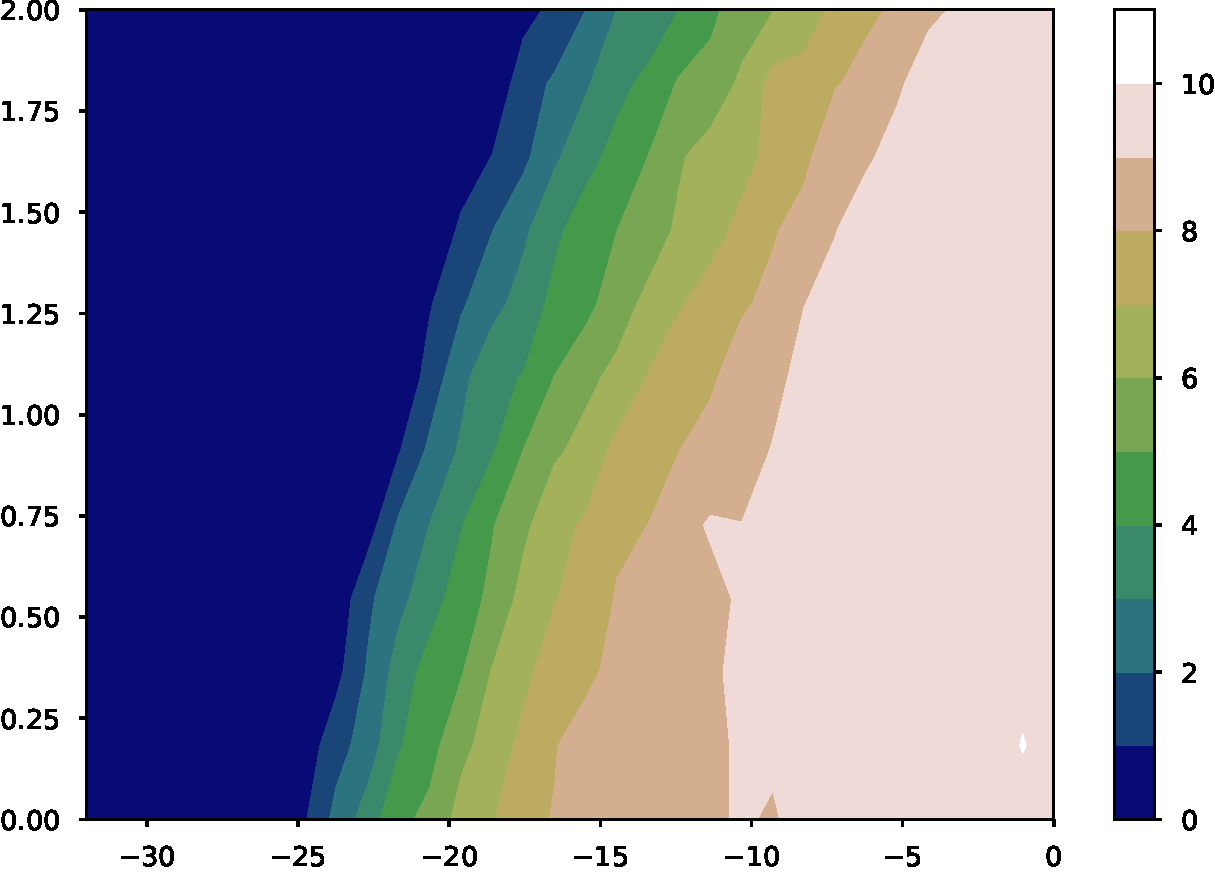
\includegraphics[width=\textwidth, height=2in]{qlr_quantile_contours.pdf}
%   \end{subfigure}
% %
%   \hfill
% %
%   \begin{subfigure}[t]{.44\textwidth}
%     \caption{QLR Statistic}
%     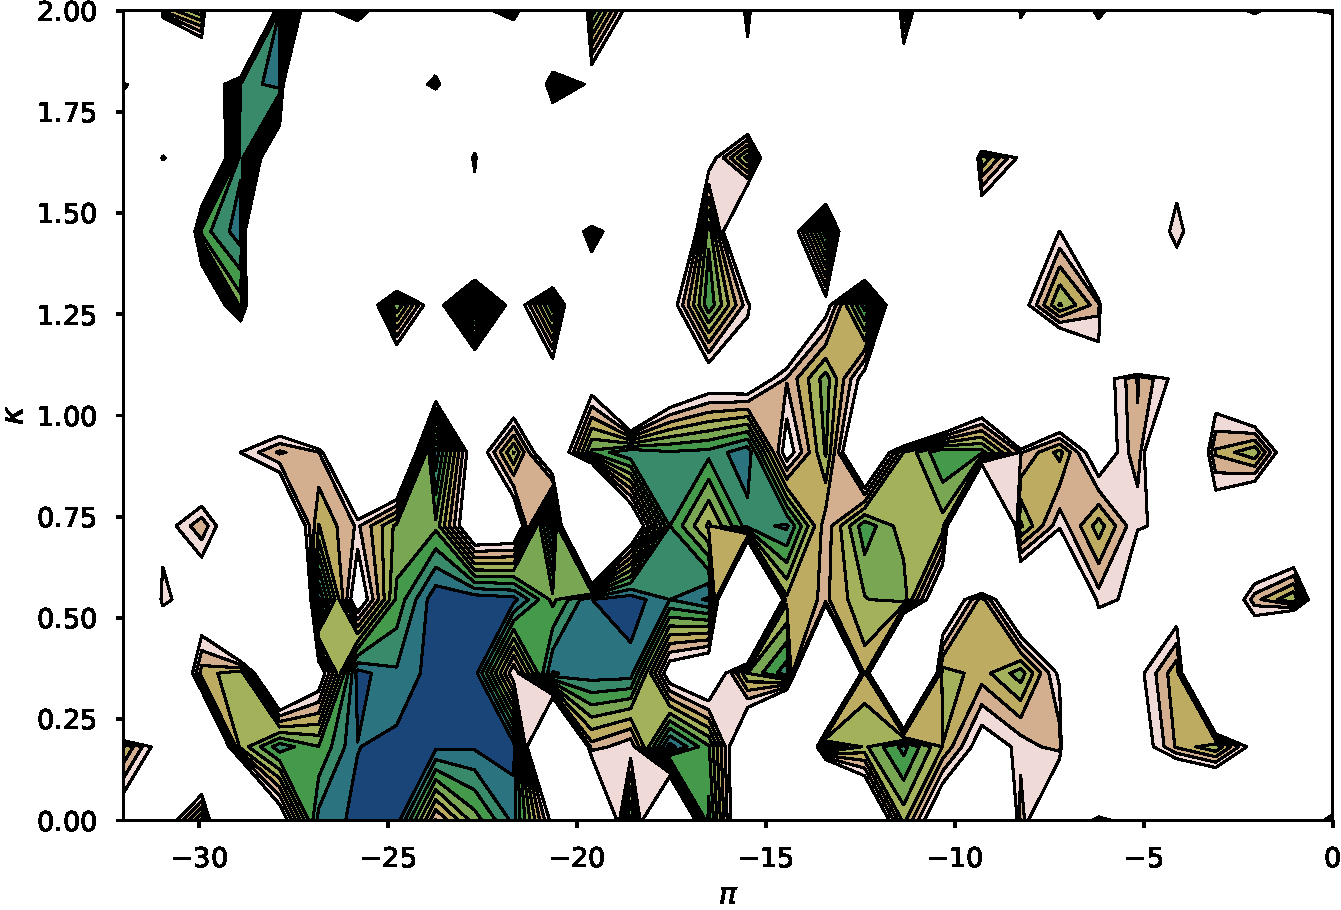
\includegraphics[width=\textwidth, height=2in]{qlr_stats_contours.pdf}
%   \end{subfigure}

% \end{figure}

